\documentclass[11pt,a4paper]{article}
\usepackage[margin=2.5cm]{geometry}
\usepackage{amsmath,amssymb,amsthm,graphicx,hyperref}
\newtheorem{proposition}{Proposition}
\theoremstyle{definition}\newtheorem{definition}{Definition}
\title{How to Know if Something is Random,\\ and if One Randomness Differs from Another}
\author{Ray Parker}
\date{October 2026}
\begin{document}\maketitle
\begin{abstract}
This note sets out Ray Parker's original framework for measuring randomness as a deviation from predictability, measured against a fixed reference called a \emph{stencil}, and for comparing two random processes by their relative deviations. It then writes up an extension Ray modelled: stacking random binary layers, whose limiting behaviour matches the Beer--Lambert law. Sections 1--2 are a faithful transcription of his handwritten notes (photos: \texttt{notes-page-1.png}, \texttt{notes-page-2.png}); text that cannot be read with certainty is marked [illegible]. The proofs and simulation in Section~3 were added when the notes were typed up.
\end{abstract}

\section{Questions and definitions}
The notes open with two questions: \emph{How do we know something is random?} and \emph{How do we know whether one randomness is different from another?}

\begin{definition}[Randomness]
Randomness $=$ deviation from predictability.
\end{definition}
\begin{definition}[Stencil]
A \emph{stencil} is a defined predictability: defined feature scores and/or ranges of expected values, against which comparisons are made, acting as an absolute reference.
\end{definition}
Both randomness and predictability are calculated against a fixed absolute reference, and in similar features. If features differ, a new temporary feature stencil is created for comparison.

\paragraph{Notation.} Let the $n$-th iteration of a defined stencil be $S_n$, and let the $i$-th randomness be $r_i$.

\section{Defined functions}
\begin{align}
\operatorname{Avg}(A,B) &= \text{average of } A \text{ and } B, \\
\Delta r_i &= r_i - S_n, \\
\operatorname{Rel}(\Delta, r_i, r_j') &= \Delta r_i - \Delta r_j' \qquad [\text{where } r_i \neq r_j'].
\end{align}
(In the notes a formula next to $\operatorname{Avg}(A,B)$ is struck out and replaced by the words ``Average of A \& B''; the bracketed condition under $\operatorname{Rel}$ is partly unclear and is read here as $r_i \neq r_j'$ [illegible: exact symbol].)

\paragraph{Stencil update.} The stencil is refined after each iteration:
\begin{equation}
S_{n+1} = \operatorname{Avg}\bigl(\Delta r_n,\ S_n\bigr),
\end{equation}
where the subscript/superscript on $\Delta r$ is partly illegible in the notes ([illegible]). If there is more than one randomness, say $K$ of them, then
\begin{equation}
S_{n+1} = \operatorname{Avg}^{k}\bigl(\Delta r_k,\ S_n\bigr), \qquad k \in [0, K],
\end{equation}
defining the given randomnesses from $r_0$ to $r_K$. Below this the notes contain a short line ``$X \to$ [illegible]'' that could not be read.

\paragraph{Matrix of stencils.} The notes then ask: \emph{what if we make a system of these stencils as a matrix, rather than calculating just one stencil for all features?} This would help manage multiple predictabilities and randomnesses separately, and also let them cross-communicate.

\section{Extension: stacked random layers}
Ray extended the framework with the following idea, which he modelled after noticing the pattern in a curtain. It is presented here as an extension Ray modelled, linking his framework to a known physical law, not as a new theorem.

Take $n\times n$ binary matrices, where $0$ is empty space and $1$ is filled space. Each layer $L_1, L_2, \dots$ is filled at random and the layers are stacked parallel to the $z$--$x$ plane along $y$. Looking from the front (along $y$), eventually no position is fully empty; yet if we ignore the count of $1$s, every position along $y$ still contains $0$s as well. Ray's conclusion: \emph{randomness extended to infinity can lead to a fixed, defined limit.}

\begin{proposition}
Suppose each cell of each layer is filled independently with probability $p\in(0,1)$. For a fixed position $(x,z)$, after $N$ layers
\[
P(\text{line of sight clear}) = (1-p)^N \to 0, \qquad
P(\text{line has at least one empty cell}) = 1-p^N \to 1 .
\]
\end{proposition}
\begin{proof}
The line at $(x,z)$ meets one cell in each layer, and these $N$ cells are independent. It is clear exactly when all $N$ are empty, which has probability $\prod_{l=1}^N(1-p)=(1-p)^N$. It is fully filled when all are filled, probability $p^N$, so it contains at least one empty cell with probability $1-p^N$. Since $0<1-p<1$ and $0<p<1$, both $(1-p)^N$ and $p^N$ tend to $0$ as $N\to\infty$.
\end{proof}
So both of Ray's observations hold together in the limit: almost every line is blocked, and almost every line still has gaps. By linearity of expectation, the expected clear fraction of the $n^2$ lines is also $(1-p)^N$.

\paragraph{Beer--Lambert law.} This is the discrete form of the Beer--Lambert law: transmitted intensity decays exponentially with thickness, $T = e^{-\mu N}$ with $\mu = -\ln(1-p)$. Ray's real-world example is graphene: a single suspended sheet absorbs about $\pi\alpha \approx 2.3\%$ of white light~\cite{nair}, an absorbance of $(2.3\pm0.2)\%$ confirmed independently~\cite{mak}. Ignoring reflection and interlayer effects, $N$ sheets transmit roughly $T\approx 0.977^N$: about $97.7\%$ for one sheet, $\approx 10\%$ for 100 sheets, and essentially $0$ for a bulk block of graphite---transparent slice, opaque block.

\paragraph{Simulation.} \texttt{sim.py} (seed 2026, $n=200$, up to 60 layers, $p\in\{0.05,0.10,0.25\}$) stacks random layers and compares the empirical fractions with theory (Figure~\ref{fig:sim}). For example, at $N=20$, $p=0.10$: empirical clear fraction $0.1222$ against theory $0.1216$.
\begin{figure}[h]\centering
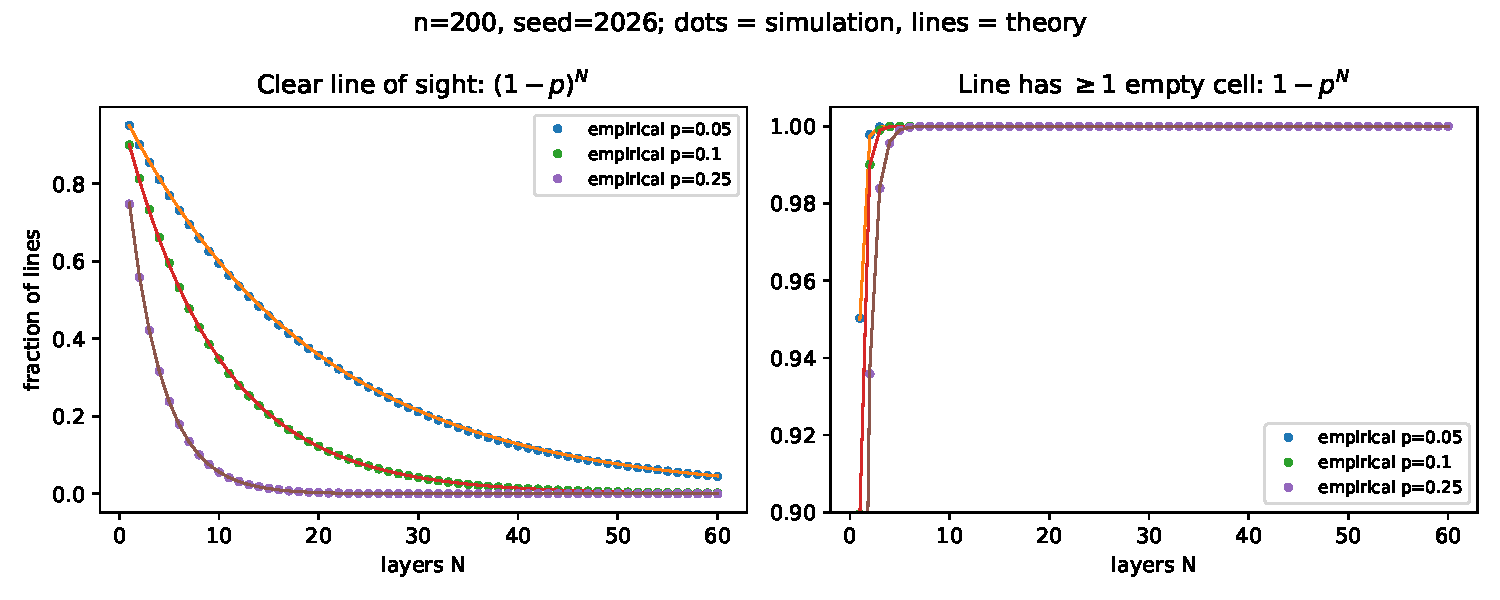
\includegraphics[width=\textwidth]{stacking_sim.pdf}
\caption{Empirical (dots) versus theoretical (lines) fractions for stacked random layers.}\label{fig:sim}
\end{figure}

\begin{thebibliography}{9}
\bibitem{nair} R.~R. Nair et al., ``Fine structure constant defines visual transparency of graphene'', \emph{Science} \textbf{320}, 1308 (2008), doi:10.1126/science.1156965.
\bibitem{mak} K.~F. Mak et al., ``Measurement of the optical conductivity of graphene'', \emph{Phys.\ Rev.\ Lett.} \textbf{101}, 196405 (2008), doi:10.1103/PhysRevLett.101.196405.
\end{thebibliography}

\appendix\section{Original handwritten notes}
\begin{center}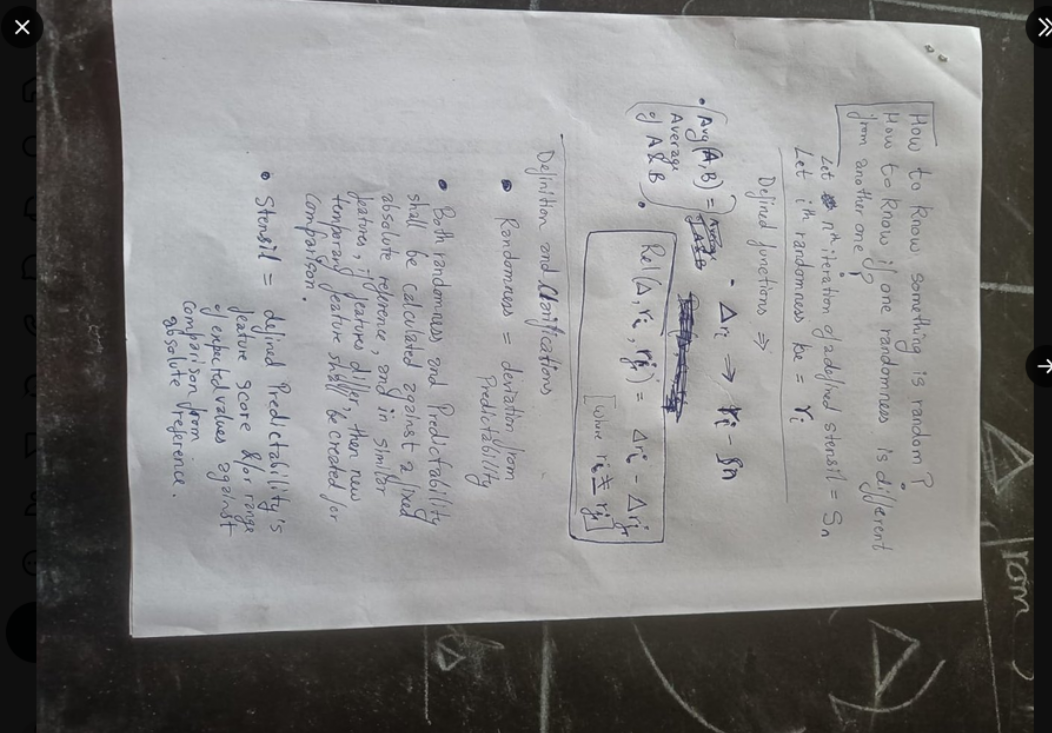
\includegraphics[width=0.8\textwidth]{notes-page-1.png}\end{center}
\begin{center}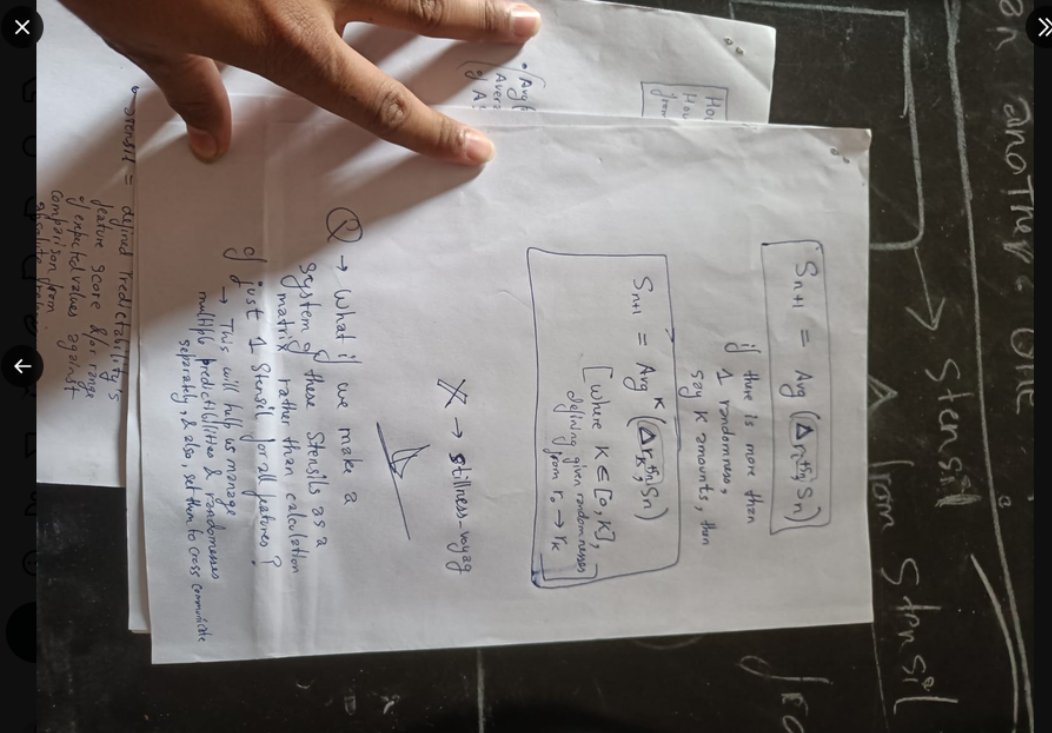
\includegraphics[width=0.8\textwidth]{notes-page-2.png}\end{center}
\end{document}
